% ==============================================================================
\section{Results}
\label{sec:results}
% ==============================================================================

\todoitem{write the results section}

%\begin{figure}[h]
%    \centering
%    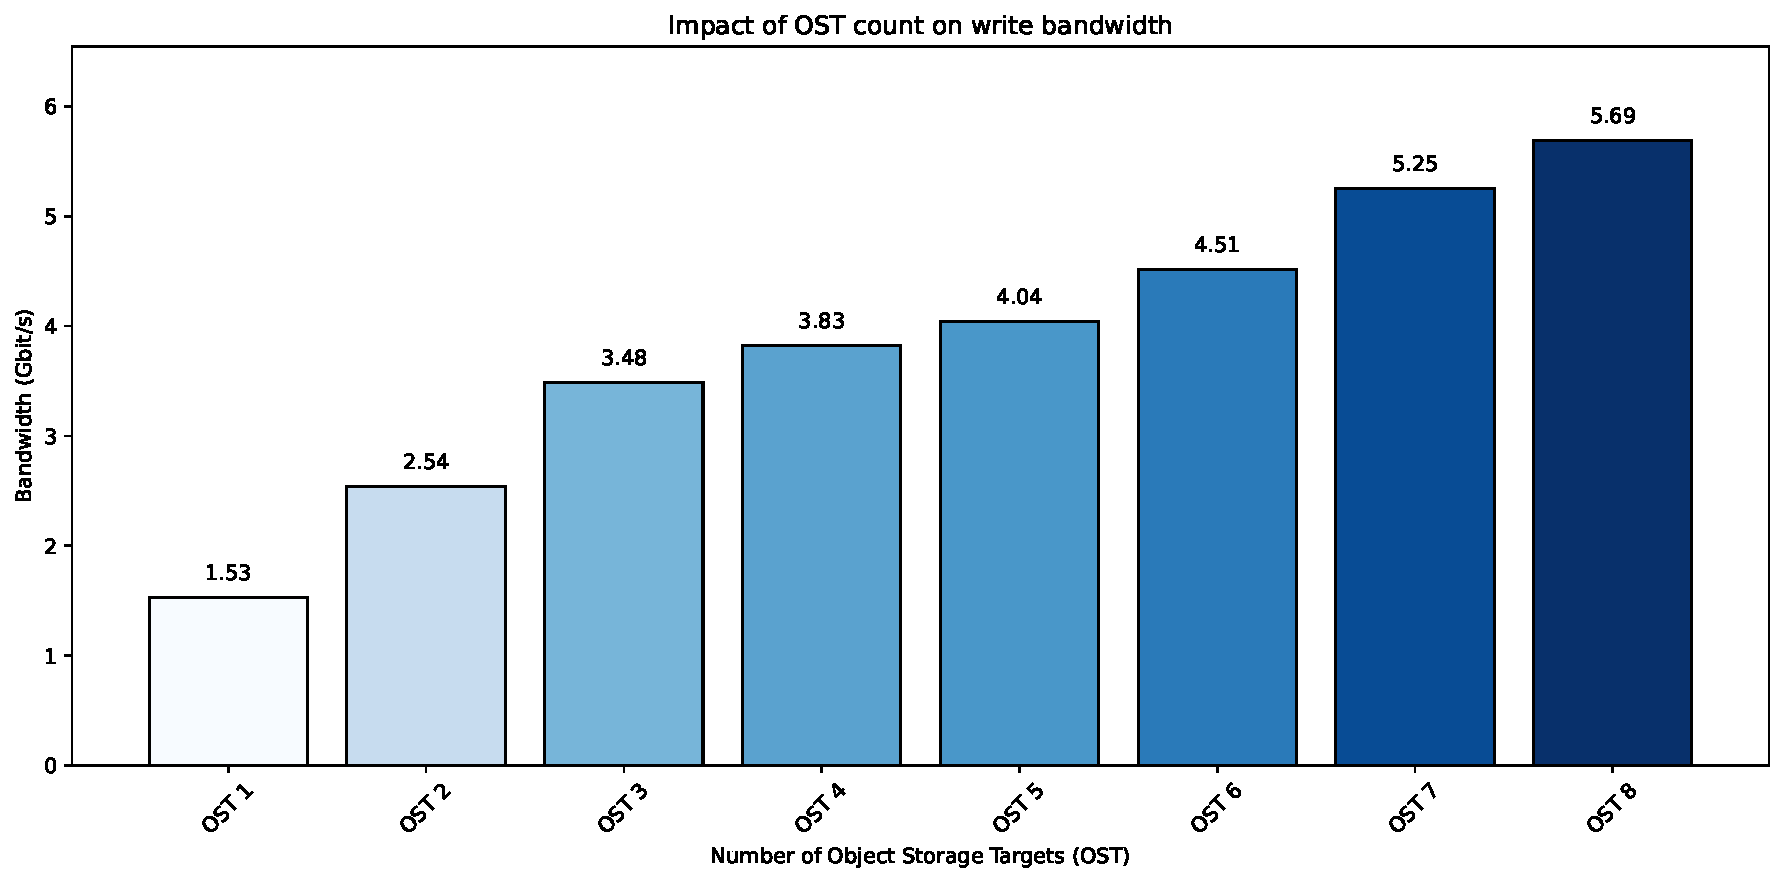
\includegraphics[width=15cm, height=6cm]{figures/results/figure_gys_io_ost_bandwidth.pdf}
%    \caption{Impact of number of OST's from 1 to 8 on bandwith on BeegFS on Plafrim}
%\end{figure}

\begin{figure}[htbp]
    \centering
    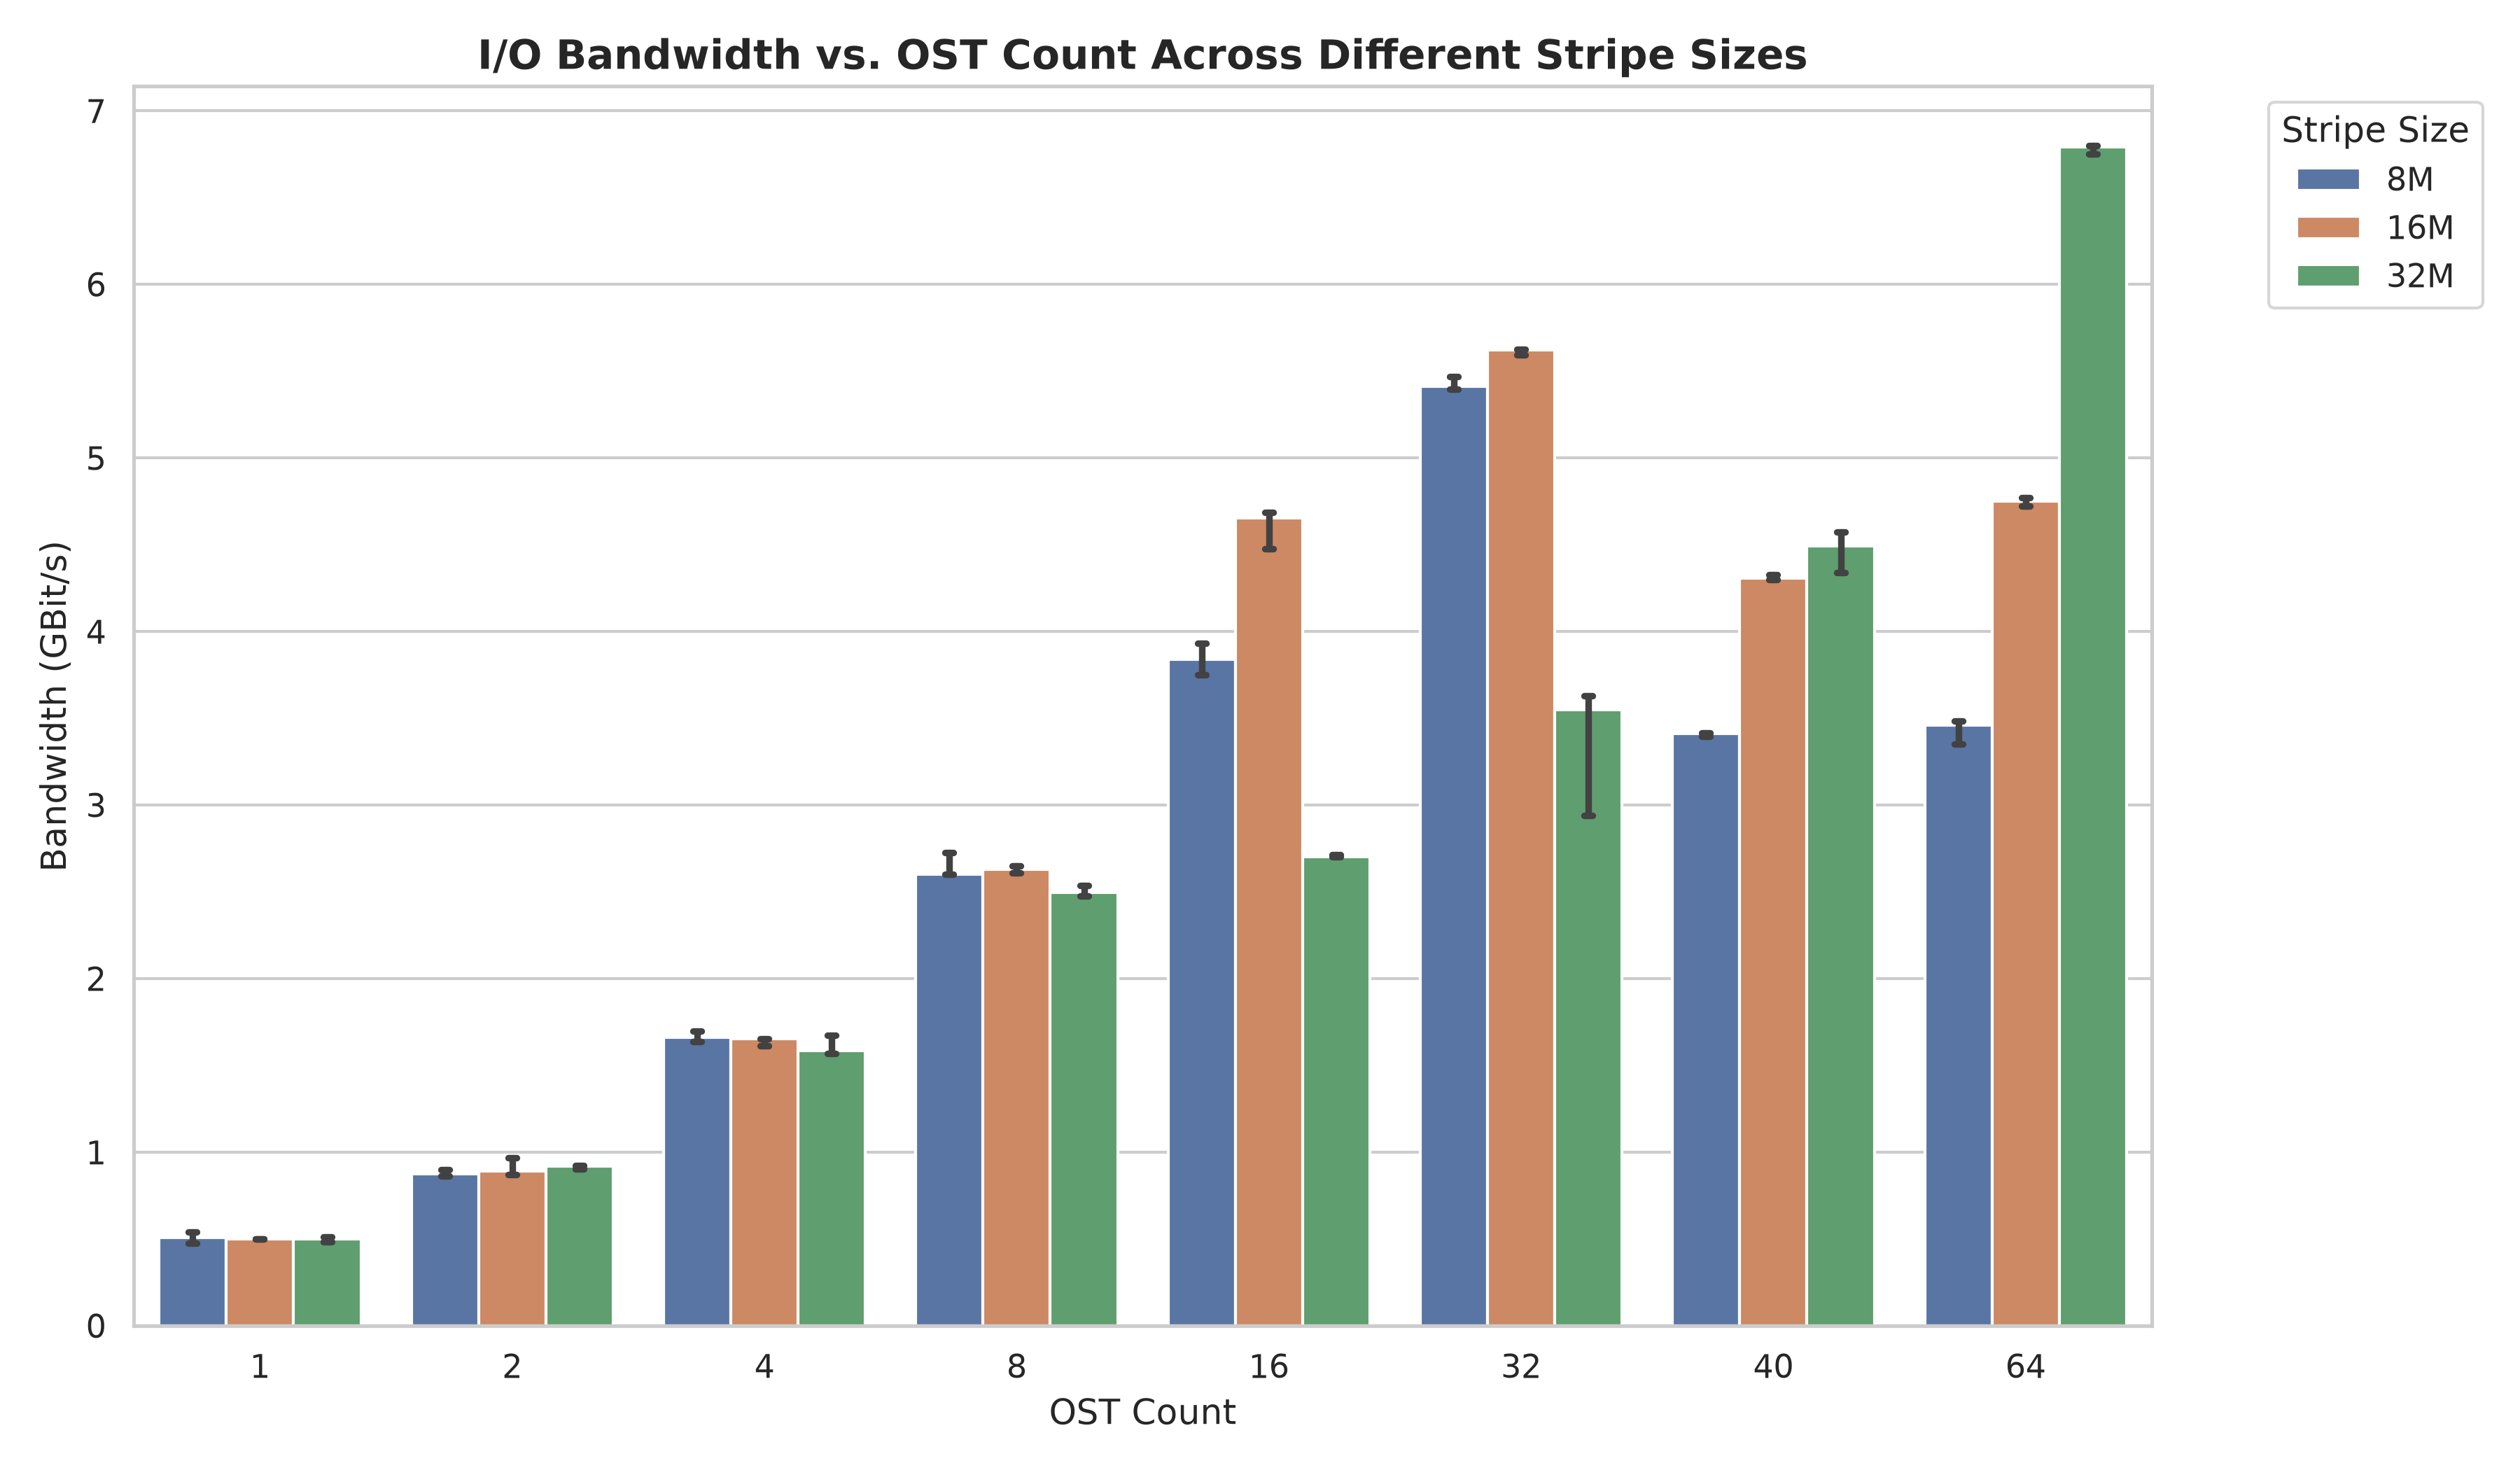
\includegraphics[width=\linewidth]{figures/bandwidth_comparaison_ost_adastra_c2.png}
    \caption{I/O Bandwidth (GBit/s) as a function of OST count (1 to 64) for different stripe sizes (8M, 16M, and 32M). Bars represent the median bandwidth, and error bars indicate the bounds/confidence interval. Performance generally scales with the number of OST, with a notable peak for the 32M stripe size configuration at 64 OSTs, reaching approximately 6.8 GBit/s, while the 8M stripe size performance plateaus or declines at higher OST counts.}
    \label{fig:bandwidth_ost_adastra}
\end{figure}

\begin{figure}[htbp]
    \centering
    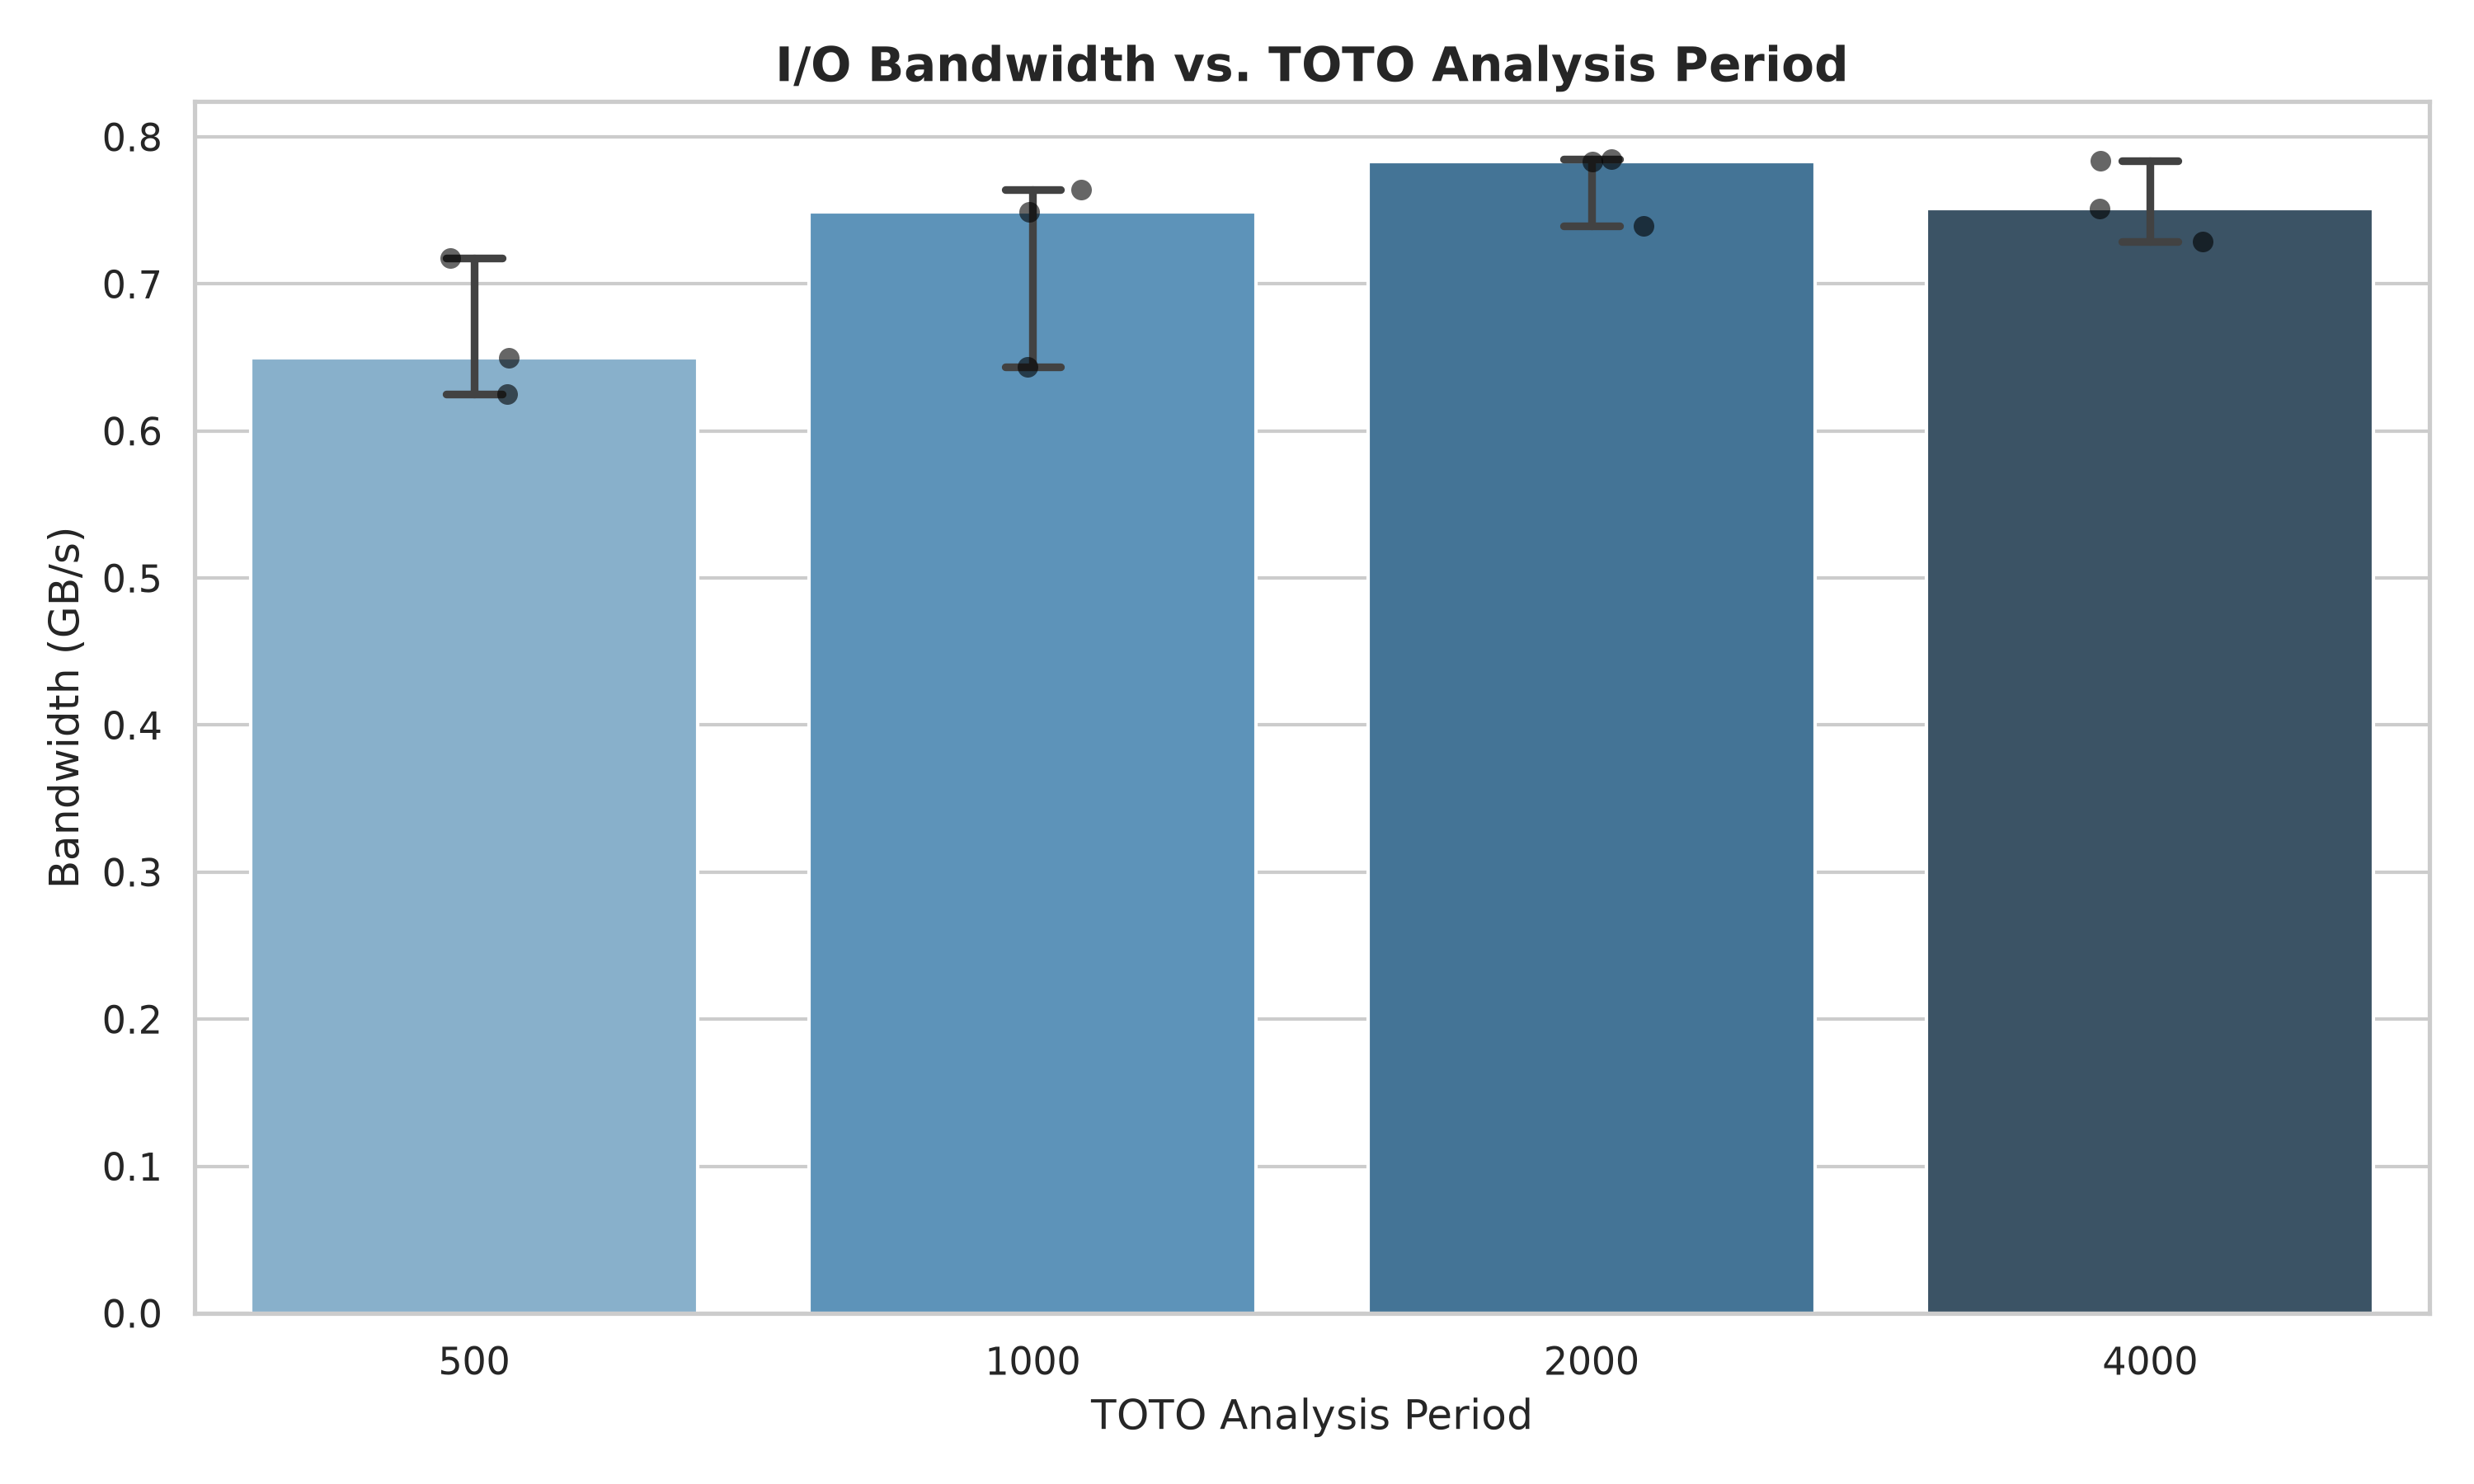
\includegraphics[width=0.85\linewidth]{figures/bandwidth_toto_analysis_period.png}
    \caption{I/O Bandwidth (GB/s) as a function of TOTO analysis period (500 to 4000). Bars represent the median bandwidth, and black dots show individual run repetitions.}
    \label{fig:toto_analysis_period}
\end{figure}